\documentclass[12pt]{article}

% Packages
\usepackage[margin=1in]{geometry}
\usepackage{amsmath, amsthm, amssymb, physics, graphicx, listings}

% Problem Box
\setlength{\fboxsep}{4pt}
\newsavebox{\mybox}
\newenvironment{problem}
    {\begin{lrbox}{\mybox}\begin{minipage}{0.98\textwidth}}
    {\end{minipage}\end{lrbox}\begin{center}\framebox[\textwidth]{\usebox{\mybox}}\end{center}}

% Options
\renewcommand{\thesubsection}{\thesection(\alph{subsection})}
\allowdisplaybreaks
%\addtolength{\jot}{1em}
\theoremstyle{definition}

% Default Commands
\newtheorem{proposition}{Proposition}
\newtheorem{lemma}{Lemma}
\newcommand{\ds}{\displaystyle}
\newcommand{\isp}[1]{\quad\text{#1}\quad}
\newcommand{\N}{\mathbb{N}}
\newcommand{\Z}{\mathbb{Z}}
\newcommand{\Q}{\mathbb{Q}}
\newcommand{\R}{\mathbb{R}}
\newcommand{\C}{\mathbb{C}}
\newcommand{\eps}{\varepsilon}
\renewcommand{\phi}{\varphi}
\renewcommand{\emptyset}{\varnothing}

% Extra Commands



% Document Info
\title{Lab 2\\
    \large GEOG 191
}
\author{Harry Coleman}
\date{January 22, 2021}

% Begin Document
\begin{document}
\maketitle

\begin{problem}
    The City of Noleta has the following minimal daily requirements for safety officials:
    \[
        \begin{array}{c|c|c}
            \text{Time (24 hour clock)} & \text{Period} & \text{Minimum number of workers required} \\\hline\hline
            2-6 & 1 & 20 \\\hline
            6-10 & 2 & 50 \\\hline
            10-14 & 3 & 80 \\\hline
            14-18 & 4 & 100 \\\hline
            18-22 & 5 & 40 \\\hline
            22-2 & 6 & 30
        \end{array}
    \]
    Each official works eight consecutive hours; someone starting in period 1 would also work in period 2. Similarly, an official starting in period 6 would also work in period 1. Let the decision variable $X_t$ represent the number of officials beginning work in each time period. The city seeks a daily schedule that employs the least number of officials, but must adhere to the stipulations established. Formulate this problem as a linear programming model, and structure and solve using Xpress-IVE.
    
    Set the model up using set notation for time periods, and coefficients as needed. Use Xpress-IVE to display the results in a custom fashion (\textit{writeln}), including decision variable values and the objective.
\end{problem}

\newpage

The total number of officials employed is the sum of the number of officials starting in each time period, i.e., our objective function is
\[
    Z = X_1 + \cdots + X_6.
\]
Let $X$ be the vector of decision variables and $c$ be the vector of coefficients given by
\[
    X = \mqty[X_1 \\ \vdots \\ X_6] \isp{and} c = \mqty[1 & 1 & 1 & 1 & 1 & 1],
\]
then $Z = cX$. We have a constraint corresponding to each of the six periods, requiring some minimum number of officials to be at work during that period. Since each official works two periods, then the officials working during a given period are those beginning work during that period and those beginning work during the previous period. Explicitly, we have the following linear constraints:
\begin{align*}
    X_1 + X_6 &\geq 20, \\
    X_1 + X_2 &\geq 50, \\
    X_2 + X_3 &\geq 80, \\
    X_3 + X_4 &\geq 100, \\
    X_4 + X_5 &\geq 40, \\
    X_5 + X_6 &\geq 30.
\end{align*}
Let $A$ be the matrix of coefficients and $b$ be the vector of coefficients given by
\[
    A = \mqty[
        1 & 0 & 0 & 0 & 0 & 1 \\
        1 & 1 & 0 & 0 & 0 & 0 \\
        0 & 1 & 1 & 0 & 0 & 0 \\
        0 & 0 & 1 & 1 & 0 & 0 \\
        0 & 0 & 0 & 1 & 1 & 0 \\
        0 & 0 & 0 & 0 & 1 & 1 \\
    ]
    \isp{and}
    b = \mqty[20 \\ 50 \\ 80 \\ 100 \\ 40 \\ 30].
\]
Then the linear constraints can, equivalently, be written as $AX \geq b$. Additionally, it is only possible to employ a nonnegative integer number of officials, so we include a sign constraint and a type constraint
\[
    X_1, \dots, X_6 \geq 0 \isp{and} X_1, \dots, X_6 \in \Z. 
\]
In terms of $X$, these constraints are $X \geq 0$ and $X \in \Z^6$. In summary, we have the following linear programming model:
\[
    \begin{array}{ll}
        \textbf{minimize}   & Z = cX \\
        \textbf{subject to} & AX \geq b, \\
                            & X \geq 0, \\
                            & X \in \Z^6.
    \end{array}
\]

\newpage
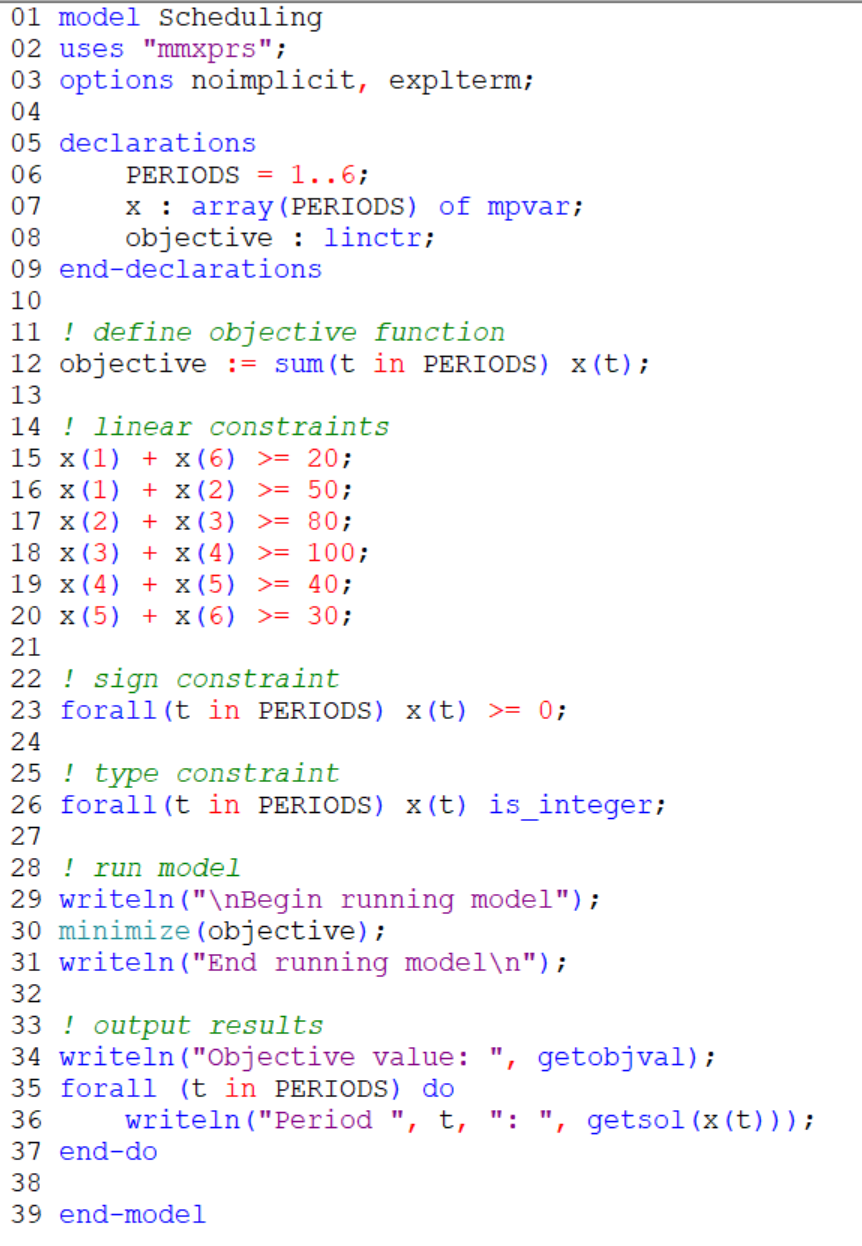
\includegraphics[scale=0.8]{code.png}

\lstset{basicstyle=\ttfamily}
\begin{lstlisting}
    Objective value: 180
    Period 1: 0
    Period 2: 50
    Period 3: 70
    Period 4: 30
    Period 5: 10
    Period 6: 20
\end{lstlisting}

\newpage
Because we have a schedule satisfying the constraints with $180$ employees, then the minimum total number of employees necessary is no more than $180$. And since Xpress says that this solution is optimal, there is no schedule with fewer than 180 employees which satisfies all constraints. Therefore, 180 is the minimum number of employees necessary to maintain schedule requirements. 

Before running the model, we could have found an upper and lower bound for this minimum. For example, having the number of employees starting in a given period equal to the minimum required for that period (i.e. $X_1 = 20, X_2 = 50, \dots$) would give a feasible solution. This gives us an upper bound of $320$ on the minimum total employees. On the other hand, if we assume that it is possible to schedule employees such that each period is exactly at its minimum, then there would have to be exactly $160$ employees. This is because each employee works for two periods and the minimum amount of employee-labor required is $320$. This would give us a lower bound of $160$ on the minimum number of employees required. However, we know from the solution to the model that $180$ is the actual minimum.

In this solution, all periods are exactly at their minimum requirements except for period 3, which has a surplus of $40$ employees. However, this is not necessarily the only optimal solution, there could be a large number of equivalently optimal solutions with different distributions of employees across the schedule.



\end{document}